\section{Body size distribution}


\subsection{Body size trends in Neogene tortoises}
%\subsection*{Genetic composition of alpine \protect\textit{Lycaeides} }

\begin{frame}
\begin{enumerate}
\p Body size distribution of Testudinidae?
\bigskip

\p \textcolor{gray}{
 Body size differences on spatial/temporal scale? 
%--> or rather continuous gene flow or all 3 species arose from one shared ancestor?
\bigskip
\p General body size trends? }
\end{enumerate}
\end{frame}


%Results1
\begin{frame}{Body size distribution - complete data set}
\begin{center}
	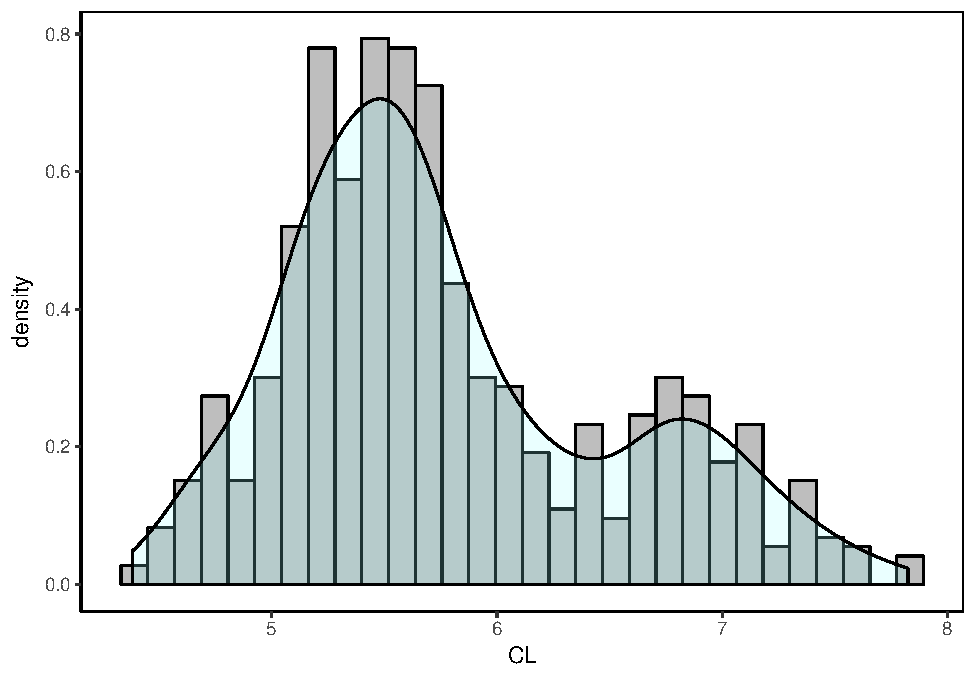
\includegraphics[width=0.75\textwidth]{MA_JJ_files/figure-latex/HistAll-1.pdf}
\end{center}

- bimodal distribution
- right-skewed: small body sizes are more frequent
\end{frame}


\begin{frame}{Body size distribution - subsets}
\begin{center}
	%\begin{figure}[htbp]
		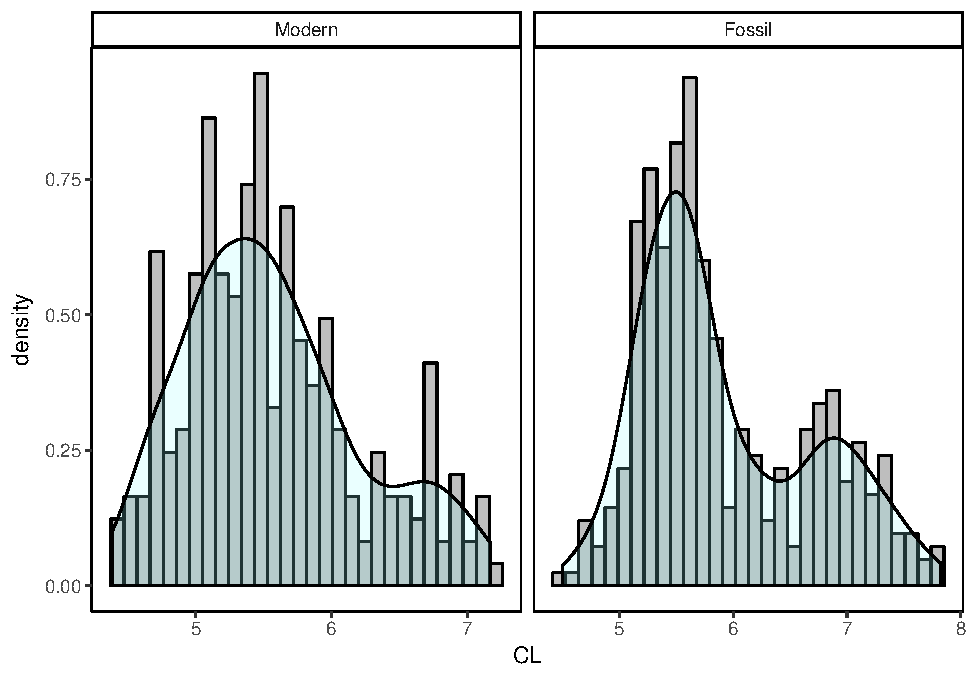
\includegraphics[scale=0.3]{MA_JJ_files/figure-latex/HistFosMo-1.pdf}
		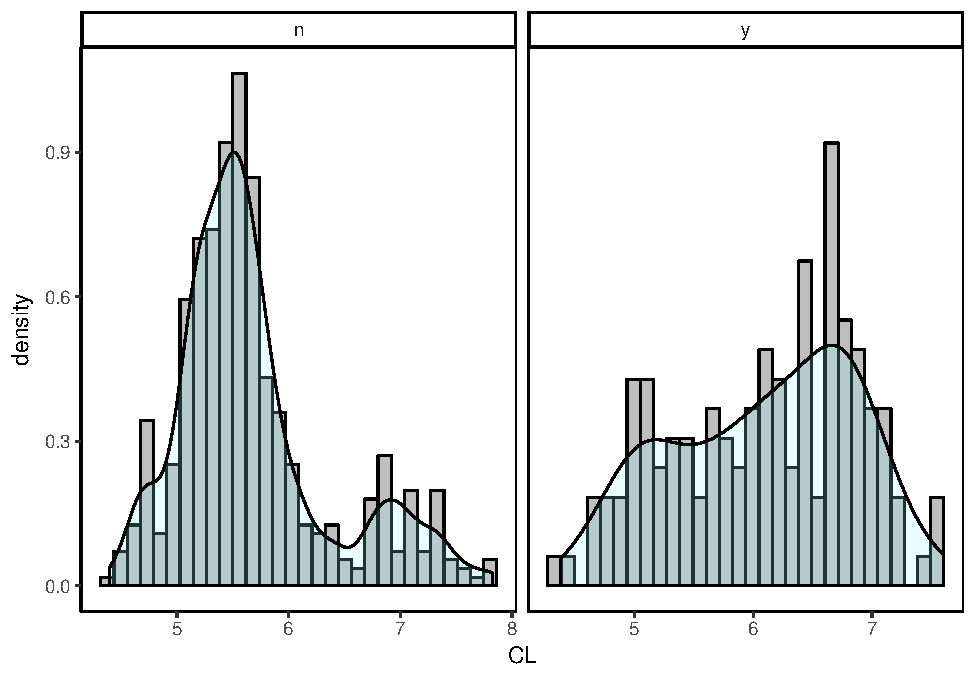
\includegraphics[scale=0.3]{MA_JJ_files/figure-latex/HistCI-1.pdf}	
	%\end{figure}
	
\end{center}

- islands: higher abundance of larger-bodied tortoises (left-skewed)
\end{frame}


\begin{frame}
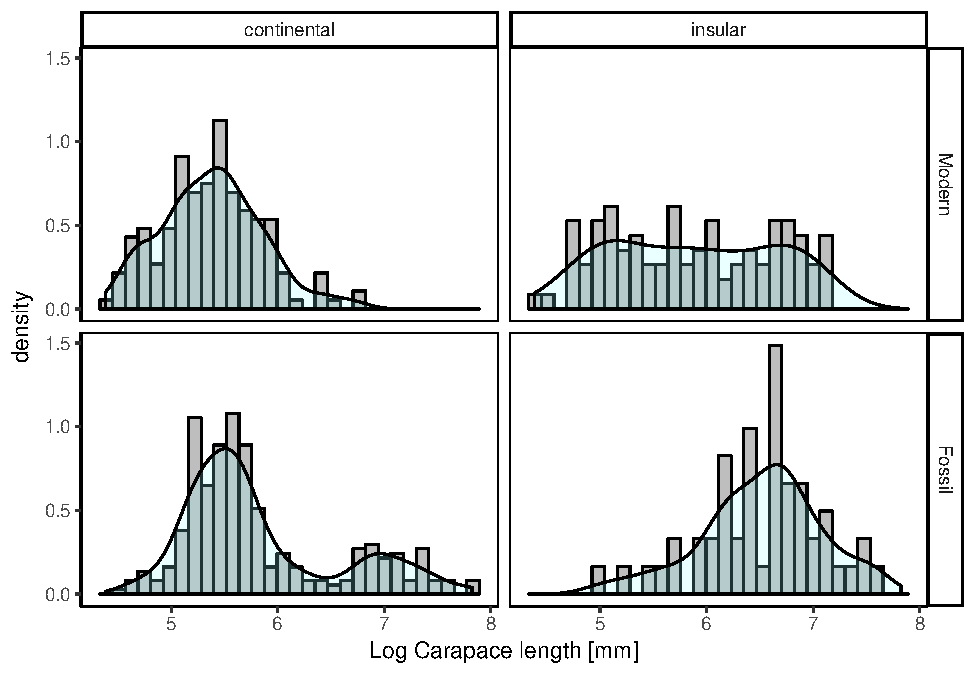
\includegraphics[scale=0.45]{MA_JJ_files/figure-latex/HistFMCI-1.pdf}

- modern continentals: no large taxa!
\end{frame}

\begin{frame}
- right-skewed body size distributions frequent in animal record: smaller animals usually more abundant - WHY? (competition, take up less space, need fewer resources, shorter generation times etc.)

- left-skewed on islands: island rule?
(has been found for turtles in other studies \pf Angielzcyk + Jaffe??)

- relatively constant through time
\end{frame}

%Discussion1


% % % % % % % % % % % % % % % % % % % % % % % % % % % % % % % % % % % % % % % % %

\section{Differences}
% on spatial/temporal scale


\begin{frame}
\begin{enumerate}
	
	\p \textcolor{gray}{Body size distribution of Testudinidae?}
	\bigskip
	\p Body size differences on spatial/temporal scale?
	%--> or rather continuous gene flow or all 3 species arose from one shared ancestor?
	\bigskip
	\p \textcolor{gray}{General body size trends?}
\end{enumerate}
\end{frame}


\begin{frame}{Comparison across time bins}
\begin{center}
	%\begin{figure}[htbp]
	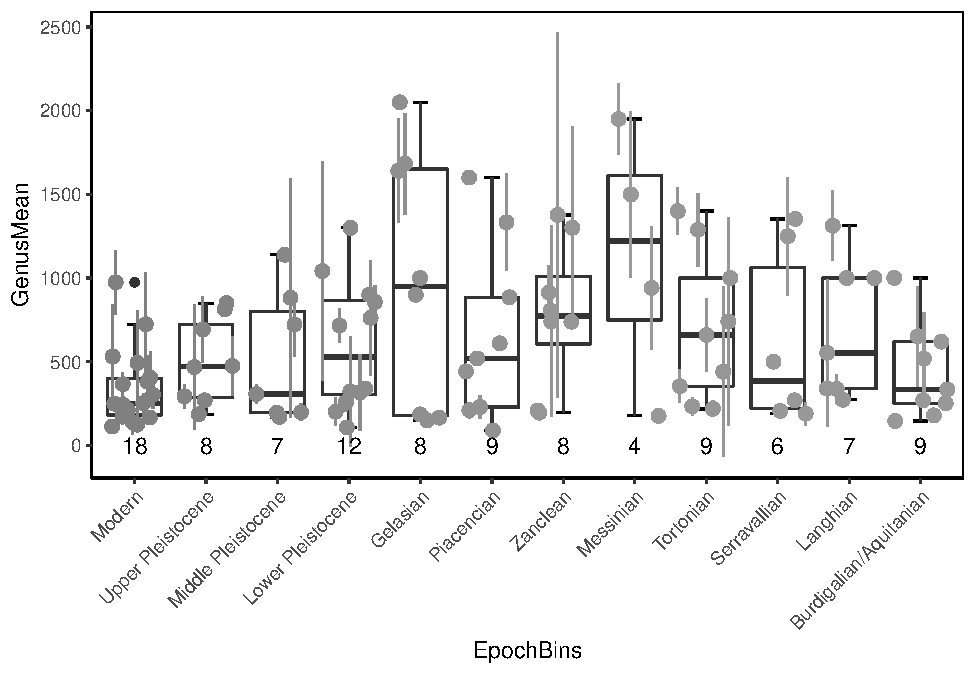
\includegraphics[width=0.9\textwidth]{MA_JJ_files/figure-latex/BPGBins-1.pdf}
	%\end{figure}
	
\end{center}

- only significant differences:
Modern $<$ Upper Pleistocene, (Serravallian $<$ Langhian)
\end{frame}



\begin{frame}{Modern $<$ fossil, continental $<$ insular}
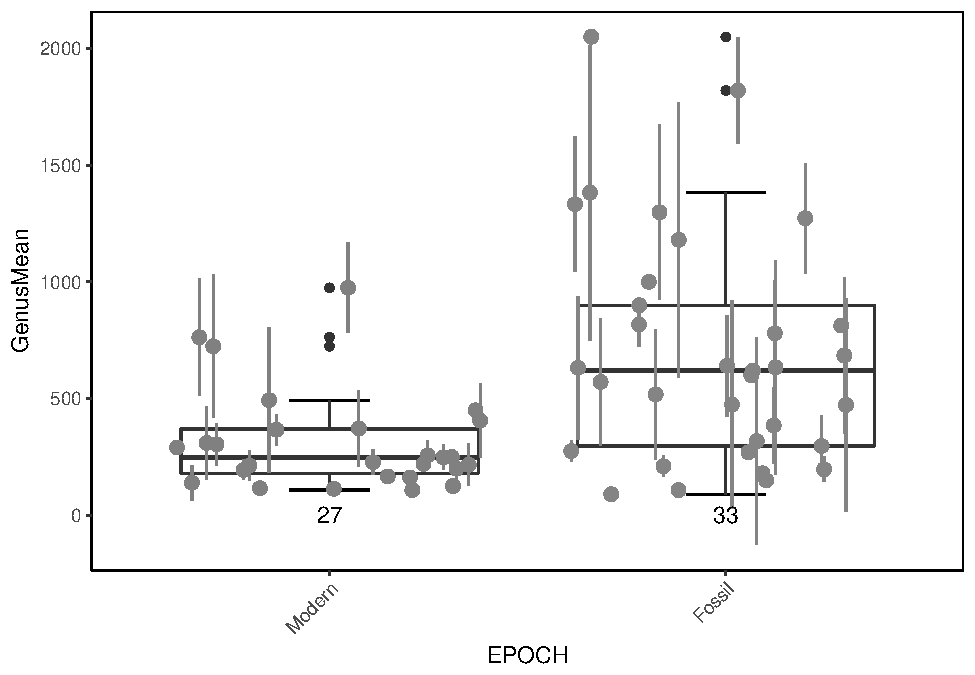
\includegraphics[scale=0.3]{MA_JJ_files/figure-latex/BPMF-1.pdf}
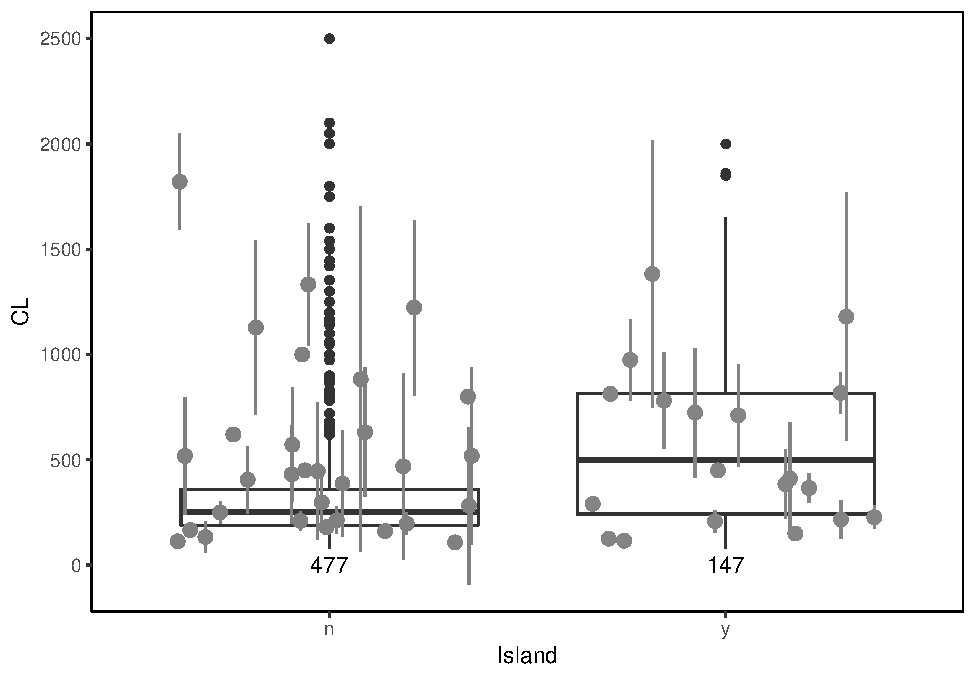
\includegraphics[scale=0.3]{MA_JJ_files/figure-latex/BPCI-1.pdf}


\end{frame}


\begin{frame}
\begin{center}
	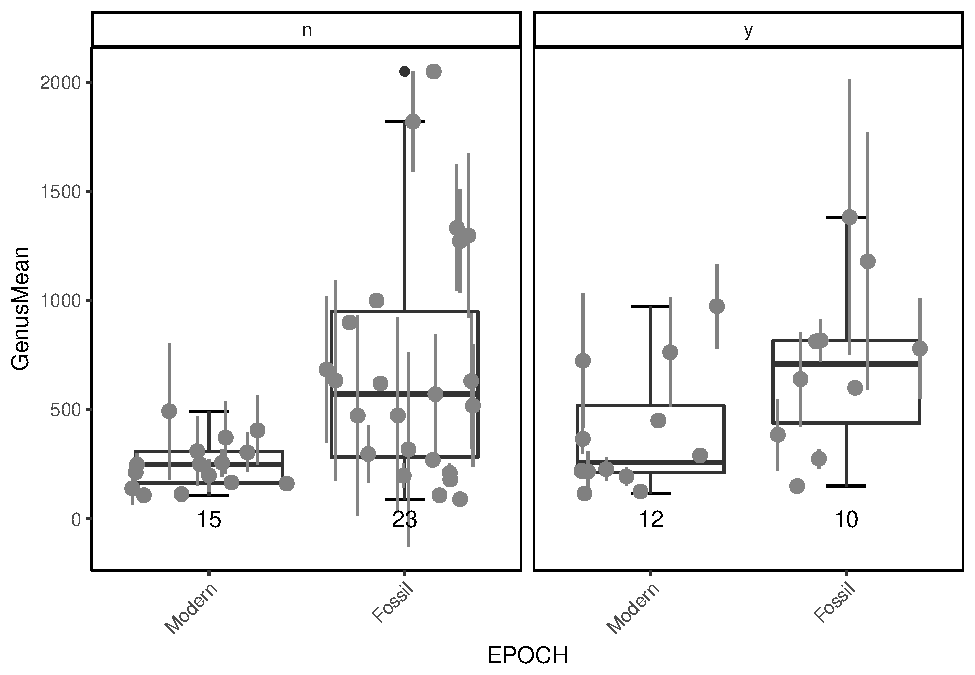
\includegraphics[width=0.75\textwidth]{MA_JJ_files/figure-latex/BPFMCI-1.pdf}
\end{center}

\end{frame}
%Results2

%Discussion2




% % % % % % % % % % % % % % % % % % % % % % % % % % % % % % % % % % % % % % % % %
\section{Body size trends}

\begin{frame}
\begin{enumerate}
	
	\p \textcolor{gray}{Body size distribution of Testudinidae?
		\bigskip
		\p Body size differences on spatial/temporal scale? }
	%--> or rather continuous gene flow or all 3 species arose from one shared ancestor?
	\bigskip
	\p General body size trends?
\end{enumerate}
\end{frame}


\begin{frame}
\begin{center}
	\includegraphics<1>[width=0.75\textwidth]{MA_JJ_files/figure-latex/paleoTScombined1.pdf}%[width=0.75\textwidth]
	\includegraphics<2>[width=0.75\textwidth]{MA_JJ_files/figure-latex/paleoTScombined2.pdf}%[width=0.75\textwidth]
	\includegraphics<3>[width=0.75\textwidth]{MA_JJ_files/figure-latex/paleoTScombined3.pdf}%[width=0.75\textwidth]
\end{center}
	
\end{frame}



